\documentclass[output=paper,modfonts,nonflat,newtxmath]{langsci/langscibook}
\author{Rafael Salaberry\affiliation{Rice University}}
\title{The conceptualisation of knowledge about aspect: From monolingual to multilingual representations}
\abstract{The theoretical dissociation between prototypical and non-prototypical conceptualisations of aspect is predicated on the effect of broad levels of contextualisation of aspectual meanings (e.g. adverbial phrases, discursive grounding). Such dissociation creates a difficult challenge for the acquisition of aspect among adult L2 learners, thus providing an ideal testing ground for the analysis of the effect of distinct sources of linguistic knowledge (i.e. the L1 and the L2) on the acquisition of aspect in the L3. In the present chapter, I review the few empirical studies on the acquisition of L2/L3 aspectual knowledge to support the claim that processing constraints associated with L2/L3 acquisition are distinct from the processes linked to the L1 acquisition of conceptualisations of aspect. I conclude that the proper identification of the theoretical construct of aspect (narrow versus broad) may have important consequences for the evaluation of models of crosslinguistic influence in general.}

\shorttitlerunninghead{The conceptualisation of knowledge about aspect}
\begin{document}
\maketitle

Most definitions of aspect focus on the speaker’s perspective about the temporal description of an eventuality, thus making such conceptualisation of situations an important component in a description of aspectual knowledge. \citet[5, italics added]{Michaelis1998}, for one, describes “aspectual categorisation as a product of the manner in which people, as producers and processors of texts, \textit{construe scenes, rather than as a reflection of the properties which situations have ‘in the world’}.” Such a perspective-driven conceptualisation of aspect is even more complex once we consider the wide range of linguistic representations, not just among first language (L1) users, but among second language (L2) and third language (L3) users (i.e. bilinguals and multilinguals). Not surprisingly, current research has not yet fully addressed theoretical questions about the representation of aspect. For instance, the variability in contextualised interpretations among not just non-native speakers, but among native speakers as well raises important questions that have not been coherently addressed by most theoretical descriptions (\citealt{Salaberry2008, Ziegeler2008, Sasse2012}). Compounding the challenge of modeling adequate representations of aspect, there have been very few empirical studies that have addressed the nature of the representation of aspect among multilinguals (e.g. \citealt{Salaberry2005, Foote2009, DiaubalickGuijarro-Fuentes2016}), even though such analysis may be crucial to assess the relevance of the construct of aspect in descriptions of (mostly) monolingual speakers.

Accordingly, the main claim to be made in this chapter is that the problem space created by a semantico-syntactic-discursive construct of such complexity as aspect provides an ideal opportunity to evaluate the multifaceted effect of previous languages (i.e. L1 and L2) on the development of the L3. This is mostly relevant in terms of assessing the two dimensions that have been identified in the theoretical models that have gathered the largest amount of empirical data in the field: the typological effect of previous languages, and the processing mechanisms used to acquire the L1 and/or the L2. To that effect, in the first section of this chapter I outline the challenges brought about by the acquisition of aspect to identify the complex and dynamic configuration of factors that affect the conceptualisation of this semantico-syntactic-discursive construct in the L1 and the L2/L3. In the second section, I briefly review some of the most representative theoretical claims proposed to account for crosslinguistic influence (CLI) in L3 acquisition in general. The main theoretical tenets of those proposals are assessed in \sectref{sec:salaberry:3} in the context of the acquisition of aspectual configurations in the L3. The analysis of the findings from the few empirical studies available on the topic is useful to evaluate the relative effect of (psycho)typological processes associated with the processing of L2 versus L1 data.

\section{Aspect} %section 1
\label{sec:salaberry:1}

%subsection 1.1.
\subsection{Lexical and grammatical aspect}
\label{sec:salaberry:1.1}

Aspect refers to the visualisation and conceptualisation of the temporal structure of situations or eventualities (\citealt{Comrie1976, Dahl1985, Smith1997}). Aspectual meanings can be categorised into two distinct layers of representation: situation type (or lexical aspect) and viewpoint (or grammatical aspect). Situation type is most commonly associated with the inherent lexical aspectual value of verbal predicates. \citet{Vendler1967} classified verbal predicates according to their inherent semantic meanings into four types: states (durative, non-dynamic, atelic), activities (durative, dynamic, atelic), accomplishments (durative, dynamic, telic) and achievements (non-durative, dynamic, telic). This classification of lexical aspect has been instrumental in the development of hypotheses about the acquisition of aspectual knowledge. The lexical aspect hypothesis (LAH, \citealt{Andersen1991}), as an example, is based on the claim that the acquisition of L2 learners’ abilities to recognise and mark aspectual configurations will happen sequentially along a developmental path that is defined by basic aspectual meanings (which are assumed to be in direct correlation with lexical aspectual values). The emphasis of the LAH is on the initial stages of the process, leaving unexplained more idiosyncratic markings based on expanded contexts of reference expected to occur in more advanced stages. This is not surprising given that lexical aspect is just one of the components in a comprehensive definition of aspect. In contrast with the plethora of studies brought about by the LAH and other similar proposals focused primarily on the effects of lexical aspect, few empirical L2 studies have addressed the more complex conceptualisation of the higher level of grammatical aspect given the need to incorporate a broader level of contextualisation into the task (see following section).

Whereas lexical aspect focuses on ontological distinctions expressed by verbal predicates, grammatical aspect makes reference to speakers’ (and hearers’) perspectives on the aspectual nature of situations and it is explicitly marked on verbal morphology. For instance, in the Romance languages the most commonly discussed contrast brought about by grammatical aspect is the use of perfective and imperfective past tense morphology. Whereas the perfective focuses on changes of state, the imperfective focuses on the permanence of the state in the world (\citealt{Klein1994,CaudalRoussarie2005}). Given its reliance on changes of state, the basic meaning of the perfective is associated with boundedness and may refer to the beginning and/or end of a situation, thus it may be inceptive, punctual or completive (e.g. \citealt{Depraetre1995}). The previous summary offers a simplified description of the construct of grammatical aspect, given that when contextualised against a larger piece of discourse, aspectual meanings convey more complex representations than the ones summarised above. As an example, \citet[156]{Binnick1991} points out that “[t]he imperfect[ive] has continual, habitual, and generic uses in many languages, while the perfect[ive] has punctual, iterative, and resultative uses.”

\subsection{Levels of conceptualisation of aspect}%subsec1.2
\label{sec:salaberry:1.2}


Aspect is a construct that is inherently defined by varying levels of contextualisation. The more decontextualised (i.e. context-poor) the situation is, the more likely it is that selections of perfective and imperfective markings will be guided by prototypical selections associated with frequency effects (for both lexical and grammatical aspect). In the absence of contextual support, interpretations about aspect rely on the basic meanings provided by lexical aspect and some minimal expansion beyond the verbal predicate. But, once we add more layers of contextual support (i.e. from a semantics-based definition we expand to a discursive one) the intersection of various pieces of information creates a complex contextual setting against which non-prototypical interpretations of aspectual meanings are more likely to occur (cf. \citealt{Binnick1991,Doiz2002}). \figref{fig:salaberry:1} provides a graphical representation of the way these various layers of aspectual representations are interrelated.

\pgfdeclarelayer{background}
\pgfdeclarelayer{foreground}
\pgfsetlayers{background,main,foreground}

\begin{figure}
\small
	\tikzset{
		treenode/.style = {
			shape=rectangle,
			rounded corners,
			draw,
			align=center,
			anchor = west,
			fill= white,
			minimum height=1cm},
		normal/.style  = {treenode, minimum width=2cm},
		lastlevel/.style = {treenode, minimum width=3cm},
		}
\begin{tikzpicture}
			[
				grow=right,
				level 1/.style={sibling distance=4cm, level distance = 3.5cm},
				level 2/.style={sibling distance=2cm, level distance = 3cm}, ]
%tree diagram
		\node (A) [normal] {aspect}
			child { node (G) [normal] {grammatical}
				child { node (P2) [lastlevel] {non-prototypical} }
				child { node (N2) [lastlevel] {prototypical} }
			}
			child { node (L) [normal]{lexical}
				child { node (P1) [lastlevel]{non-prototypical} }
			child { node (N1) [lastlevel]{prototypical} }
			};
% Background Rectangles
	\begin{pgfonlayer}{background}
		\node[fit = (P2) (N2) (P1) (N1), rectangle, rounded corners, inner sep = 0.3cm, fill = gray!20] (R3) {};
		\node[fit = (P2) (N2) (P1) (N1), rectangle, fill = gray!20, rounded corners, inner sep = 0.3cm, left = 0.8cm of R3] (R2) {};
		\node[fit = (P2) (N2) (P1) (N1), rectangle, fill = gray!20, rounded corners, inner sep = 0.3cm, left = 0.8cm of R2] (R1) {};
	\end{pgfonlayer}
%"Titles" of columns/Rectangles [V2]
	\node (C3) at (N1) [above = 2.5\baselineskip,anchor=base] {Context};
	\node (C2) at (C3.base -| L) [anchor=base] {Components};
	\node (C1) at (C3.base -| A) [anchor=base] {Construct};
\end{tikzpicture}
\caption{\label{fig:salaberry:1}Graphical representation of layers of aspectual conceptualisation}
\end{figure}
%

The following examples from Spanish depict the complex nature of non-pro\-to\-typi\-cal aspectual\largerpage interpretations of state verbal predicates brought about by the informational context provided by specific adverbial phrases.\footnote{Examples are from \citet[102]{Guell1998}.}

\ea \label{ex:salaberry:1}
\begin{xlist}
    \ex \label{ex:salaberry:1a}
    \gll Lo supo               / *sabía              durante mucho tiempo.\\
         it know.\textsc{pret} {} know.\textsc{ipfv} during much time  \\
    \glt  ‘(S/he) knew it for a long time.’

    \ex \label{ex:salaberry:1b}
    \gll Lo *supo / sabía  desde hacía mucho tiempo.\\
    it know.\textsc{pret} {} know.\textsc{ipfv} since ago much time\\
    \glt ‘(S/he) knew it from a long time ago.’

\end{xlist}
\z

First, the non-prototypical use of the preterite (\textsc{pret}) with a state verb in \REF{ex:salaberry:1a} presented in conjunction with the adverbial \textit{durante mucho tiempo} prevents an inchoative interpretation (i.e. the beginning of the state), bringing about an aspectual meaning typically reserved for the imperfective form (i.e. non-punctual, durative; \textsc{ipfv}). But, notice that the imperfective form is dispreferred (marked with an asterisk) in \REF{ex:salaberry:1a}. Along the same lines, the preference for the imperfective form in \REF{ex:salaberry:1b} stands out in this context given the use of an adverbial phrase that, in principle, would trigger an inchoative interpretation. The imperfective choice maintains the focus on the actual state irrespective of the explicit highlighting of the inception point (the perfective form is dispreferred).\footnote{See \citet{Doiz2002} for an expanded discussion of this complex description of aspectual contrasts in Spanish.}

An example of the complex nature of grammatical aspect is provided by the distinct meanings conveyed by the aspectual (contrastive) concepts of iterativity and habituality (e.g., \citealt{deSwart1998, Langacker1999}). In general, iterativity conveys the basic idea of the repetition of specific eventualities (focus on the episodic nature of eventualities), whereas habituality is akin to generic statements that focus on the overarching concept that an eventuality has been iterated (emphasis on the generalisation of the iteration). In the Romance languages, perfective and imperfective forms are used to describe the iteration of eventualities: iterativity and habituality are conveyed with the use of Spanish preterite and imperfect, respectively. In principle, whereas the imperfect prototypically conveys the aspectual notion of habituality (as shown in \ref{ex:salaberry:2a}), the preterite conveys a rather distinct aspectual concept, the notion of iterativity \REF{ex:salaberry:2b}.

\ea \label{ex:salaberry:2}
\begin{xlist}
\ex Habitual\label{ex:salaberry:2a}\\
\gll {Cuando} {era} {niño,} {Lucas} {jugaba} {al} {fútbol}.\\
When was child Lucas played at.the football\\
\glt  ‘When [he] was a child, Lucas played/used to/would (\textsc{imp}) play soccer.’
\ex Iterative\label{ex:salaberry:2b}\\
\gll Lo *supo  / sabía  desde hacía mucho tiempo.\\
it know.\textsc{pret} {} know.\textsc{ipfv} since ago much time\\
\glt ‘For years, Lucas played (\textsc{pret}) soccer.’
\end{xlist}
\z


As was the case in the example described above, the specific effect of the adverbial phrase triggers distinct aspectual meanings (i.e. habituality or iterativity) that transcend the simple prototypical meanings of boundedness assigned to the imperfective-perfective contrast (e.g. \citealt{SlabakovaMontrul2007, Scholes2008,Salaberry2013}).

\subsection{{Linear} {and} {non-linear} {patterns} {of} {development}}
\label{sec:salaberry:1.3}

The theoretical dissociation between prototypical and non-prototypical representations of aspect brought about by the complex nature of aspectual meanings at both the level of lexical and grammatical aspect presents a challenge for the analysis of the acquisition of aspect. That is, empirical studies may focus on invariant (prototypical) or, alternatively complex (non-prototypical) meanings, thus generating possibly contradictory results across studies.

To showcase the distinct outcomes prompted by different procedures of data collection, I summarise the results of two studies focused on the acquisition of iterativity in L2 Spanish among L1 English speakers, both offering converging evidence on the separation of two types of knowledge about aspect. In the first study, \citet{SlabakovaMontrul2007} analysed the grammaticality judgments of English native speakers who were L2 Spanish classroom learners (27 advanced learners and 33 intermediate learners) and 27 native Spanish speakers on the use of the perfective marker with single or multiple events (punctuality versus iterativity). Overall, the results showed that, on the one hand, the judgments of all learners were indistinguishable from the responses of native speakers on the punctual interpretation of the perfective (prototypical meaning). On the other hand, there was a significant difference between learners and native speakers on the judgments of iterative interpretations (non-prototypical). In the second study, \citet{Scholes2008} replicated the findings from Slabakova and Montrul with learners of similar levels of experience and he also included an additional group of near-native speakers (graduate students teaching Spanish). Both studies also included a traditional fill-in-the-blanks test that assessed the basic use of past tense morphology focusing on the aspectual concept of perfectivity (original test used in \citealt{Salaberry1999}).

The graphical representation of the converging findings from both studies is shown in \figref{fig:salaberry:2} (based on data from \citealt{Scholes2008}).

\begin{figure}
    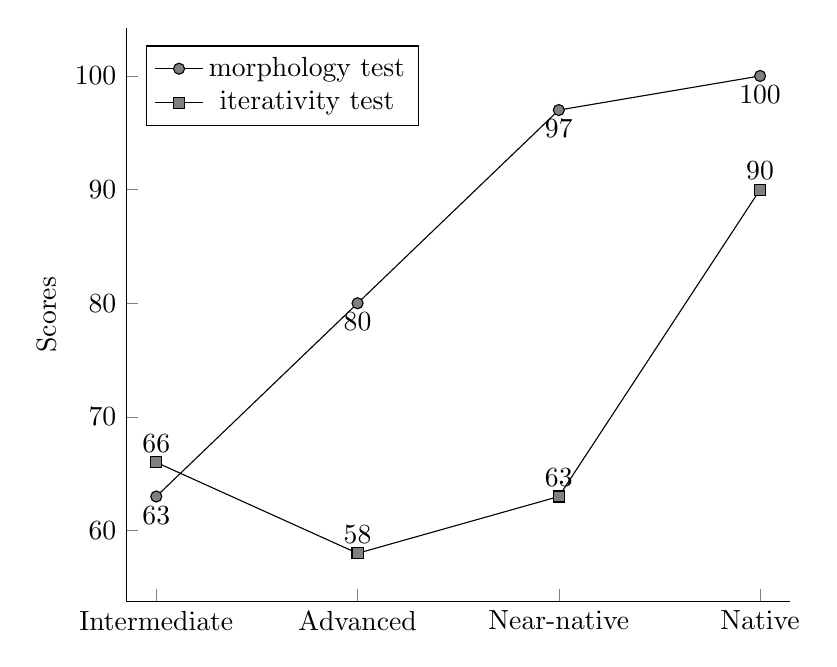
\begin{tikzpicture}
    \begin{axis}[
    scale only axis,
    enlarge x limits=0.05,
    ylabel = Scores,
    xtick = {1,2,3,4},
    xticklabels = {Intermediate, Advanced, Near-native, Native},
    axis lines*=left,
    nodes near coords,
    legend pos = {north west},
    cycle list name=black white,
    ]
     \addplot+[nodes near coords align={below}] table {
        x   y
        1   63
        2   80
     	3   97
       	4   100
       };
       \addplot+[]  table {
       		x   y
      		1   66
      		2   58
       		3   63
      		4   90
       		};
    \legend{morphology test,iterativity test}
    \end{axis}
    \end{tikzpicture}
    \caption{\label{fig:salaberry:2}Development of perfective (prototypical) versus iterative (non-prototypical) meanings}
\end{figure}


The developmental trajectory for the prototypical linguistic representations of aspect in Spanish past tense morphology (63\%, 80\% and 97\%) – as measured by the responses to the fill-in-the-blanks task – shows a gradual and constant increase in the form of a linear pattern in parallel with increased experience with the L2 (intermediate, advanced and near-native). In contrast, the results from the test of iterativity show no such linear development according to proficiency level. In the iterativity test, all non-native speakers remain within the range of 50--60\% of correct responses, which is very close to chance level. We can tentatively conclude that the access to instructional activities with a metalinguistic focus on sentence-level aspectual markers leads to constant progress towards the overall use of preterite and imperfect in the context of prototypical realisations of aspect. Arguably, the lack of access to similar metalinguistic focusing activities for non-prototypical contexts of the concept of aspect may, in principle, be responsible for the lack of progress. It is also possible that no amount of instructional effort placed on the identification of (and practice with) non-prototypical representations of aspect in the L2 may be sufficient for learners to incorporate such nuanced descriptions of aspect.

In sum, the theoretical dissociation between prototypical and non-prototypical conceptualisations of aspect is predicated on the effect of broad levels of contextualisation of aspectual meanings (e.g. effect of adverbial phrases, discursive grounding). Such dissociation happens at the levels of both lexical and grammatical aspect (e.g. non-inchoative meanings of states with perfective morphology or the concept of iterativity in contrast with habituality), creating a difficult challenge for the acquisition of aspect. The L2 studies reviewed above provide some initial empirical evidence that substantiates the above-mentioned claim.

\section{{Disambiguating} {the} {concept} {of} {cross-linguistic} {influence}} %section 2
\label{sec:salaberry:2}

The previous discussion of the complexity of the concept of aspect brought about by multi-layered representations of various meanings associated with aspectual knowledge is useful to assess the main postulates of hypotheses that have modeled the effect of language transfer or CLI. The latter is defined as “the influence resulting from the similarities and differences between the target language and any other language that has been previously (and perhaps imperfectly) acquired” \citep[27]{Odlin1989}.

Given that the L3 is preceded by more than one language, the search for the identification of CLI on L3 learning is multi-faceted \citet{DeAngelis2007} and should be assessed, at a minimum, along three separate dimensions. First, there are several linguistic factors, such as typological similarities (e.g. \citealt{Rothman2011, Rothman2015, WestergaardEtAl2017}), psychotypology (e.g. \citealt{Kellerman1983, BardelLindqvist2007}) and conceptual semantic primitives (\citealt{BermanSlobin1994, Slobin1996, BerkesFlynn2012}) that can influence CLI. Second, there are methodological factors that are likely to influence transfer, such as proficiency level (e.g. \citealt{Dewaele2001, DeAngelis2007, Lindqvist2010}), recency of use of the given languages (e.g. \citealt{WilliamsHammarberg1998}) and order of acquisition effects (e.g. \citealt{Dewaele1998, WilliamsHammarberg1998}). Finally, language transfer may differ in the L2 and/or the L3 depending on which type of distinct learning process (e.g. declarative versus procedural knowledge) may be used as the conduit for any type of linguistic influence to materialise.

The majority of previous CLI models have focused primarily on the factors identified by the first two dimensions of analysis reviewed above (i.e. linguistic and methodological factors). The dimension of learning process has become the main component of one particular model: the L2 status factor (\citealt{BardelFalk2007, BardelFalk2012, FalkBardel2010, FalkBardel2011}). It should be noted, however, that the relevance of processing factors to guide the acquisition of the L3 still represents an important component of other models, albeit indirectly. For instance, \citet[9]{BerkesFlynn2012} assume, a priori, a specific type of cognitive processing of language data (i.e. UG-guided). That is, in their model, the structural typological makeup of any (source or target) language “reflects the way that language-specific CP [complementiser phrase] develops within the constraints of UG.” Other proposed models such as the typological primacy model (TPM, \citealt{Rothman2011, Rothman2015}) are similarly based on a UG-guided model of acquisition. To properly assess the combined effect of linguistic and methodological factors on the one hand, and learning processes on the other hand, I will review the proposals made by three theoretical models that have been claimed to account for CLI on the L3: The cumulative enhancement model (CEM), the TPM, and the L2 status factor model.\footnote{Apart from lack of enough empirical data, some recent proposals represent expansions of basic tenets of previous models selected for review above. For instance, \citet{Slabakova2017} builds upon the CEM and the TPM proposals to add specific acquisition constraints (e.g. acquisition of properties one by one and the effect of non-facilitative transfer). Similarly, \citet{WestergaardEtAl2017} expand on the effect of linguistic typology (on a property-by-property basis, unlike the TPM) and add the factor of abstract structural similarities (while also allowing for both facilitative and non-facilitative effects, unlike the CEM).} The selection of only three models is partly based on the fact that the identified models have been supported with a fairly significant empirical database, and in part due to the inclusion of the independent variables to be discussed in this chapter (i.e. typology and learning process) among the main theoretical tenets of such models.

\subsection{{Linguistic} {and} {methodological} {factors} {behind} {CLI}} %2.1.
\label{sec:salaberry:2.1}

The CEM posits that knowledge from previous languages creates a multiplying positive effect to guide the development of a third language (on a property-by-property basis) (e.g. \citealt{BerkesFlynn2012, FlynnEtAl2004}). More specifically, \citet[7]{BerkesFlynn2012} propose that “[a]ll previously known languages are available to the learner to constructively enhance subsequent language learning.” Not only does this model eschew any categorical distinction between the L1 and the L2 for the development of a third one, but it also contends that the combined information from all previous languages contributes to the learning process in a positive way. The latter position contrasts with previous deficit models of CLI based on constructs such as interference and negative transfer that impeded and slowed down the acquisition process (see \citealt{Odlin1989}). The CEM regards such constructs as irrelevant for the development of a language that is guided by universal grammar precepts, explicitly conceptualising any perceived negative transfer as part of temporary performance phenomena. On the other hand, it should be noted that \citet[1--2]{BerkesFlynn2012} claim that the construction of a new grammar on the part of the learner can be made more effective (i.e. efficient cognitive processing) if learners are provided with information about “what does not have to be taught,” and more importantly, about the syntactic primitives that are needed for the learner to process the L3 “in a new and economical way.”

The TPM can be framed within the general claim of the full transfer/full access hypothesis proposed by \citet{SchwartzSprouse1996}. It is based on a cognitive economy principle predicated on reducing the cost of processing language transfer from the already existent language systems into the L3 (e.g. \citealt{Rothman2011, Rothman2015}). Within this model, actual and perceived typological and structural similarities between the L3 and both the L1 and the L2 will be used to guide and facilitate the acquisition of the L3. Three additional tenets of the TPM provide an expansion of this basic principle of cognitive efficiency. First, \citet[180]{Rothman2015} argues that transfer happens “holistically, that is, not on a structure-by-structure basis.” Second, this overriding economy principle entails that neither the L1 nor the L2 would have any preferred status to become the source of language transfer. Third, the holistic restructuring of the L3 happens early in the acquisition process. The TPM’s foundational notion – that learning any additional language carries cognitive processing costs and that learners, in principle, will use a selective process to transfer language information from previous languages based on cognitive economy – is rather uncontroversial. On the other hand, the additional tenets described above have been challenged both at the theoretical and the empirical level. From a theoretical perspective, \citet{Slabakova2017}, for instance, contends that the TPM’s overarching focus on the initial state of acquisition of the L3 limits its explanatory value. She argues that wholesale transfer need not be more economical in terms of cognitive processing: “Why would the LAD/parser expend resources on blocking off some cross-linguistic influence that may turn out to be profitable later on?” (2017: 658).

As already stated, the two models of CLI highlighted above can be described as models that address, primarily, two main dimensions of analysis: the characteristics of languages previously learned (i.e. typology) and specific methodological factors (e.g. stages of acquisition of languages other than the L1).

\subsection{Types of knowledge in L3 processing}%2.2
\label{sec:salaberry:2.2}\largerpage
The third model to be summarised here, the L2 status factor model, most clearly identifies the role of distinct types of knowledge as a central factor for the development of the L3. Given that this paper is focused on the effect of types of knowledge, this third model will be described in more detail than the previous two. The L2 status factor model is predicated on the notion that the type of cognitive processing required to learn the L3 is more similar to the processing conditions required to learn the L2 rather than the L1 (e.g. \citealt{WilliamsHammarberg1998, BardelFalk2007, FalkBardel2011, BardelSánchez2017}). The initial claim about a qualitative difference in processing associated with previous languages stems from the analysis of empirical data carried out by \citet[323]{WilliamsHammarberg1998}: “provided the factors of proficiency, typology and recency are at a sufficient level, L2s appear more likely to be activated than the L1 as supplier language during the early stages of L3 acquisition.” Following up along that line of thought, \citet{FalkBardel2011} remarked on some similarities shared by the L2 and L3 acquisition processes: age of onset, learning outcome, learning conditions, and more importantly, the level of awareness of the learning process (including degree of metalinguistic knowledge and the use of learning strategies). A corollary of this position is that learners rely on two systems to process language information: “two separate knowledge bases working side by side without interaction” (\citealt{FalkEtAl2015}:  228). Eventually, \citet{BardelFalk2012} explicitly tied previous empirical findings and related theoretical claims to the development of a neurolinguistic framework of analysis that was tied to the declarative/procedural model from Paradis (2009) and others.\footnote{The emphasis on the nature of the processing of linguistic information in the L3 does not entail that the L1 may not influence the process. For instance, \citet{FalkEtAl2015} point out that whenever learners increase their metalinguistic awareness and knowledge of their L1, such information may become part of the information fed into the L3 system under development.}\largerpage

Given the focus of the L2 status factor model on the assessment of relative levels of cognitive similarity of language processing between the L3 and prior non-native languages, it is important to describe two parallel theoretical contrasts predicated on the notion of awareness that separate distinct types of processing of linguistic information: the declarative-procedural and explicit-implicit dichotomies. \citeauthor{Anderson2013} (2013, inter alia) contrasts the knowledge of factual information (declarative) from the knowledge of how to perform skills (procedural). For his part, \citet[269]{Williams2005} defines implicit knowledge as achieved without the intention to learn, and, more importantly, without awareness of what has been learned, whereas explicit knowledge is prompted by situations in which learners intend to learn and are aware of what they have learned.\footnote{There are, however, important differences between these two contrasts. \citet{Ullman2016}, for instance, points out that the declarative-procedural memory system is based on empirical evidence from brain functions, whereas the explicit-implicit contrast is based on studies of psychological awareness that are very difficult to test empirically. Furthermore, Ullman notes that these contrasts are not isomorphic, given that the declarative memory system can underlie both explicit and implicit knowledge, whereas the procedural memory system is associated with implicit knowledge only (p. 959).} The non-interface position between these two types of knowledge was forcefully put forward by \citet{Krashen1985} in the form of two strong postulates: acquisition and learning are distinct theoretical constructs, and second and more importantly, conscious, explicit learning of the L2 cannot lead to its (unconscious, implicit) acquisition (see also \citealt{Schwartz1993, AthanasopoulosEtAl2015}, for early support of Krashen’s position). More recently, \citet[63]{Paradis2009}, using neurolinguistic evidence, also rejected the claim of any type of interface via conscious access to the mental state that underlies proceduralised knowledge: “During the appropriation of an L2, the use of competence may replace the use of metalinguistic knowledge over time, […]. This is not an interface but the substitution of the use of one mechanism for the use of another.” Along the same lines, \citet[956--957]{Ullman2016} proposes that the declarative and procedural memory systems can “acquire the same or analogous knowledge or skills.” For that reason, they compete with each other (the constrained use of one will lead to compensation from the other one).

In contrast with the non-interface position, \citet{DeKeyser2003, DeKeyser2009} argued for a strong interface between declarative and procedural knowledge. DeKeyser’s assertion of causality is, however, qualified: ``explicit learning certainly \textit{does not necessarily lead to eventual automatized, let alone implicit, knowledge} […]'' (\citealt[126]{DeKeyser2009}, italics added). As a compromise, an intermediate position, sometimes referred to as a weak interface, has been adopted by Rod \citet{EllisR1993, EllisR2008} and Nick \citet{Ellis2005}. In general, this weak interface assumes that metalinguistic awareness and negative evidence serve as a conscious priming mechanism to lead learners to notice the gap between the input and their existing linguistic competence. In other words, metalinguistic information in the form of explicit teaching (creating declarative knowledge) may be relevant to \textit{realign} the orientation of the L2 learner towards the implicit learning of the new linguistic system. As acknowledged by Nick \citet[330]{Ellis2005}, however, the (obvious) focusing of attention through guided metalinguistic awareness is “by no means necessary” for a causal effect on implicit knowledge. In sum, the strong and weak interface hypotheses seem to focus on correlation effects, and not causality. In other words, the apparent \textit{relationship} between declarative and procedural memory systems need not entail an interface.

\subsection{Learning processes applied to aspect} %2.3
\label{sec:salaberry:2.3}

The interaction between the two knowledge systems described above (or, more precisely, their lack of interaction) is similar to the description of the acquisition of aspect along the lines of two distinct dimensions as summarised in \sectref{sec:salaberry:1}. Most notably, the separation of the implicit competence and explicit knowledge (associated with the L1 and the subsequent Lns) parallels the demarcation between non-prototypical and prototypical conceptualisations of aspect. This is most obvious in the disconnect between the results of the iterativity test describing the iterativity-habituality contrast and the results on the traditional past tense morphology test assessing prototypical perfective-imperfective contrasts. We can surmise that if there is no interface between implicit and explicit knowledge, the L1 is most relevant for the acquisition of deep conceptual components of language (non-prototypical). That is, the non-linear type of learning associated with complex aspectual concepts is representative of the type of implicit language knowledge not readily available through focused metalinguistic awareness activities (either in the L2 or the L3). In contrast, the linear process of learning documented in the studies reviewed above for the prototypical meanings of aspect shows the effects of metalinguistic information available in the L2 and the L3.

Overall, the linguistic representation of temporality is constrained by the options afforded by each language. Picking apart the effects of several contextual layers of information is complex, and for such a complicated task, the conceptualisation of aspect from the L1 seems to guide the L2 user to identify what information is relevant for the linguistic realisation of aspectual meanings. In essence, part of the challenge is due to the subtle and difficult task of noticing configurations of aspectual representations spanning over several layers of contextual information. On this point, the analysis of data on the L2 acquisition of aspect shows that the L1 acts as a filter to acquire and develop the L2 representation of temporality. For instance, \citeauthor{AthanasopoulosBylund2013}'s study (2013: 287) focused on the aspectual contrast created by diverse languages such as English or Spanish, which have “a tendency not to mention the goal or endpoint of an event when describing goal-oriented dynamic scenes,” with, on the other hand, languages like German or Swedish with “the reverse tendency, that is, a bias toward mentioning the goal of actions.” Similarly, \citet{SchmiedtovaEtAl2011} contend that the choice of temporal perspective is not random, but dependent on the aspectual configurations of the L1. Finally, \citet[116]{Bylund2011} concludes that L1 conceptualisation patterns remain strong among highly competent L2 speakers.

Arguably, it appears that conceptualisation patterns from the L1 remain central for the processing of aspectual representation even in advanced stages of acquisition of an L2. It remains open to question, however, whether targeted metalinguistic awareness tasks and correlated practice may provide L2/L3 learners with the option to integrate the meanings of non-prototypical and prototypical meanings into their L2/L3 aspectual systems. \citet{Bylund2011}, for instance, notes that the specific representation of grammatical aspect will direct a person’s attention to certain event features. Under these conditions, increased metalinguistic awareness and metacognitive skills, prompted mostly by the acquisition of the L2 (the first second language) may help learners maximise their chances of learning an L3 (at a minimum in terms of efficiency, as shown in \citealt{NayakEtAl1990}).

\section{The third language acquisition of aspect}%3
\label{sec:salaberry:3}

As mentioned above, there is a dearth of studies on the L3 acquisition of aspect. In this section, I summarise the findings from three relevant studies (restricted to adult L2/L3 learners) to assess the value of some of the theoretical claims made in previous sections regarding linear and non-linear development in association with prototypical and non-prototypical meanings: \citet{Salaberry2005, Foote2009, DiaubalickGuijarro-Fuentes2016}.\footnote{Although there is an increasing number of studies on the L3 acquisition of aspect, some are not directly relevant for the present analysis because they primarily focus on constructs of aspect that do not comprise the full range of meanings of aspectual representations (i.e. including the analysis of both prototypical and non-prototypical meanings). For instance, \citet{Fessi2013} assesses the explanatory value of the lexical aspect hypothesis, whereas \citet{KarpavaEtAl2012} focus on the validity of the Full Transfer/Full Access hypothesis (see \sectref{sec:salaberry:1} above). For reference, however, one such study focused on a limited representation of the construct of aspect \citep{Foote2009} is described in detail given that it uses the same L3 as the studies reviewed in the present section.}

The study by \citeauthor{Salaberry2005} provides information about the possible limitations on the conceptualisation of aspectual configurations based on CLI from the L2. The data from \citeauthor{Foote2009} is useful to understand the positive effects of transfer from the L1 and the L2 on the prototypical meanings of lexical aspect. Finally, the analysis by \citeauthor{DiaubalickGuijarro-Fuentes2016} provides confirmatory evidence about the apparent failure of learners to incorporate non-prototypical aspectual configurations into their grammars in both the L2 and the L3.

\citet{Salaberry2005} focused on the development of aspectual contrasts in L3 Portuguese among L1 English speakers who also knew Spanish as an L2. Both Spanish and Portuguese (as Romance languages) share the same conceptualisation of aspect, so it was expected that learners would benefit from their knowledge of the L2 to learn similar contrasts in the L3. The study was based on grammaticality judgment data collected with the use of a narrative text that was used to contextualise the use of a total of 30 verbal predicates divided into three lexical aspectual classes (13 telic events, 7 atelic events and 10 statives). Participants had to select the appropriate morphological marker (perfective or imperfective) for each verbal predicate used in the text. Not surprisingly, the overall findings revealed that the L1 English-L2 Spanish learners had achieved a high level of proficiency in the selection of past tense aspectual markers in the L3. To wit, the selection of the imperfective marker was broadly distributed across lexical aspectual classes showing a clear dissociation between lexical and grammatical aspect, attesting to the advanced knowledge of aspectual marking in the L3. Furthermore, there was an overall consistent positive trend in the selections of past tense endings to mark the dynamic classes of verbal predicates (telic and atelic events) across both native and non-native groups. There was, however, one major discrepancy between the responses of native and non-native speakers of Portuguese. When the analysis of data focused on the judgments about the category of statives only, the selection of inflectional markers of past tense among L3 Portuguese participants was less consistent and less categorical than among native speakers of Portuguese. Hence, it appears that the influence of the L1 English conceptualisation of aspectual knowledge (most noticeable on the aspectual marking of states) had an effect on the conceptualisation of non-prototypical markers of states.

\citet{Foote2009}, in turn, investigated the effect of typological similarity of a Romance language used as the L1 or as the L2 on the transfer of knowledge about aspect to another Romance language functioning as the L3. The two L1-L2 combinations used in her study were: L1 English-L2 Romance language and L1 Romance language-L2 English. Both groups were also learning an L3 which was an additional Romance language (different from the one known as an L1 or L2). Foote hypothesised that knowledge of the semantic contrast of aspectual meanings – irrespective of the status of this language as an L1 or an L2 – would transfer to the L3. The main assessment instrument used by Foote was a sentence conjunction judgment task which was intended to evaluate semantic implications based on the concept of perfectivity (i.e. focus on endpoint markers). Each sentence depicted an eventuality marked with perfective or imperfective morphology that was contradicted or not by another event marked with perfective morphology in the second part of the sentence. The use of the perfective form in the second part of the sentence prompted a consistent ungrammatical option (illogical), whereas the use of the imperfective led to a grammatical reading (logical).

Overall, the findings show that, irrespective of whether the Romance language was the participants’ L1 or L2, all L3 speakers were able to distinguish the semantic distinctions of perfectivity depicted in the test sentences. \citet[111]{Foote2009} concluded that both L3 groups “seem to have been able to transfer their knowledge from the previously known Romance language,” further stating that her data “suggest that language typology does play a role in source(s) of transfer in L3 acquisition.” By design, however, the assessment instrument used by Foote tested prototypical representations of aspectual meanings of Romance languages’ past tense morphology. Despite the fact that Foote incorporated a triad of languages to discriminate any order effect of any particular L1/L2 combination on the L3, the data collection was predicated on a limited conceptualisation of aspect. As a consequence, the complexity of a semantico-syntactic-discursive grammatical construct like aspect cannot be evaluated with an assessment instrument focused on the decontextualised meanings of aspectual contrasts.

Finally, \citet{DiaubalickGuijarro-Fuentes2016} set out to assess the knowledge of complex notions of aspectual meanings in L2 Spanish (i.e. coercion effects) among L1 German speakers. Their study is relevant for the present analysis for two important reasons. First, the majority (if not all) of the participants in the study were actually L3 Spanish learners because the German L1 speakers also knew English as an L2; their level of proficiency in L2 English was judged to be generally in the order of B1 or higher in the Common European Framework of Reference for Languages (Diaubalick, personal communication). Second, coercion effects were predicated on examples depicting the iterativity-habituality contrast reviewed above. The authors considered two hypotheses for their analysis: The interpretability hypothesis and the feature reassembly hypothesis. After the analysis of the findings, however, Diaubalick \& Guijarro-Fuentes conclude that neither one of these proposals could account for the findings of their study. In both cases, the aspectual meanings brought about by coercion of the prototypical meanings are not acquired by any of the learner groups (low intermediate, high intermediate or advanced). Diaubalick \& Guijarro-Fuentes surmise that the “uninterpretable features connected to perfectivity that are responsible for a verb rising to AspP are not acquired since even advanced speakers do not reach native level” (p. 192). With regards to the claim of the feature reassembly hypothesis they conclude that the latter “fails to explain why the differences between the German and English learners are as reported … the problems with the coercion effects, in particular, persist until late stages” (p. 194).

The results from this study replicate the findings from the studies on the concept of iterativity reviewed above: the more complex notions of iterativity and habituality were not acquired by the L1 German-L2 English speakers in their study (for the relevance of English in this case see \citealt{AthanasopoulosBylund2013} and \citealt{AthanasopoulosEtAl2015}). In the end, \citeauthor{DiaubalickGuijarro-Fuentes2016} conclude that their study may have focused on the incorrect hypotheses and surmise that “[p]erhaps the acquisition of the Spanish past tenses presents a phenomenon that is rather connected to the lexicon than to the interpretability of features” (2016: 194). This is a more plausible interpretation than the one initially considered by the authors, given that the shift from a purely syntactic definition of aspect toward a more contextualised (cf. lexical) one is more likely to focus on a more complex description of what knowledge about aspect entails in the grammar of the L1, the L2 or the L3.

The limited empirical evidence on the L3 acquisition of aspect gathered so far seems to point in the direction of a limited conceptualisation of aspect in the L2 that prevails in the process of incorporating such a theoretical construct into the L3 system. The study from \citet{Salaberry2005} was useful to address the role of non-prototypical interpretations of the lexical aspectual category of statives leading to the conclusion that the L1 representation of \textit{lexical aspect} (restricted to the limited conceptualisation of L1 English) prevailed over any possible beneficial effect of the L2 (a language that had the same representation of aspectual configurations as the L3). On the other hand, the study from \citet{DiaubalickGuijarro-Fuentes2016} provided additional converging empirical evidence to support the same claim, but with data from the acquisition of non-prototypical instantiations of \textit{grammatical aspect} (i.e. iterativity, or coercion in their description).

\section{Discussion}%4
\label{sec:salaberry:4}

In the present chapter I have brought into focus one particular construct (aspect) that can offer a viable testing ground for some of the claims made about CLI models proposed to account for the competence of both bilinguals and multilinguals. In essence, the use of aspect as the dependent variable in L3 acquisition studies provides a yet untapped context of learning that could be beneficial to (a) evaluating the nature of the development of a multilayered grammatical concept (aspect) across the L1, the L2 and any subsequent language, and (b) help elucidate the process of learning other complex grammatical concepts.

For multilingual learners who have access to two (or more) distinct sources of linguistic knowledge (i.e. the L1 and the L2), I focused on the specific analysis of two separate main effects (among many) on the processing of this complex theoretical construct: on the one hand, the specific typological structures and language information from the previous languages, and, on the other hand, the distinct way of processing linguistic information represented in the L1 and the L2. Previous models of CLI have addressed the relevance and weight of these constructs (i.e. typology or processing) in different ways, depending on various internal theoretical aspects of the frameworks that inform such CLI models. Overall, the analysis of empirical data on the acquisition of knowledge about aspect in the L3 confirms and expands on previous findings about other grammatical constructs that have been the subject of analysis of previous studies of CLI (i.e. effect of typological differences). Notwithstanding this confirmatory finding about the effect of typological contrasts, the analysis of the acquisition of the contextualised definition of aspect contributes important data to assess the effect of learning mechanisms across the L1, the L2 and the L3 in ways that other constructs have not tapped into.

The empirical data on the acquisition of aspect reviewed above show the following important findings. First, the available data on the type of learning process behind the acquisition of aspect in the L3 seems to indicate that the L3 system will rely on the same processing mechanisms that were used to develop the L2, inheriting in the process both the advantages and the limitations of that knowledge system. This is most clearly represented in the linear progression of aspect marking in prototypical settings demonstrating a positive correlation between improvement in aspect marking and experience with the target language (i.e. a main feature of explicit learning mechanisms). Second, despite the previous assertion, the influence of the (psycho)typological stock of the L1 for the acquisition of aspectual configurations (e.g. \citealt{Bylund2011, SchmiedtovaEtAl2011, AthanasopoulosEtAl2015}) seems to account for apparent discrepancies between native and non-native speakers. As demonstrated in the analysis of data of several studies, whenever aspectual meanings are the product of multiple layers of contextualisation (i.e. non-prototypical representations), there is an L1 effect across all subsequent languages. That is, for the acquisition of non-prototypical meanings of aspect at least, neither the L2 nor the L3 (processed in qualitatively different ways than the L1) can overcome the limitations of learning processes to re-conceptualise a construct (i.e. aspect in its full complex representations) that seems to be dependent on L1 processing mechanisms.

The most interesting outcome of the present analysis of the L3 acquisition of aspect is given by the apparent far-reaching effect of the L1-based conceptualisation of aspect on the development of the L3 representation of this complex construct. While, in principle, one could argue that this is evidence against the L2 status factor model, the opposite is actually the case. More precisely, the failure of L3 users to access the processing system that was part of the L1 acquisition process confirms the proposed reliance of the L3 acquisition mechanism on the L2 developmental infrastructure.  This provides confirmatory evidence for the main claim of the L2 status factor model: the L1 and L2 represent distinct processing mechanisms with the L3 matching the characteristics of the L2 system. When the L2 system is not able to tap into L1 processing mechanisms, the L3 will also fail to access the L1 processing mechanisms. In sum, the basic claim of the L2 status factor of a distinction in terms of language processing may be most relevant for the evaluation of a comprehensive definition of aspect that includes a representation of distinct levels of conceptualisation of aspectual knowledge. Additional studies teasing apart the effects described above in different language combinations would provide empirical evidence that could attest to the empirical viability of the analysis of the currently available proposal that was summarised in this paper.

{\sloppy\printbibliography[heading=subbibliography,notkeyword=this]}
\end{document}
